\documentclass{book}
\usepackage[spanish]{babel}
\usepackage[utf8]{inputenc} 
\usepackage[T1]{fontenc}
\usepackage{lmodern}
\usepackage{graphicx}
\usepackage{amsmath}
\usepackage{xcolor}
\usepackage{verbatim} 
\usepackage{enumerate} % enumerados

%\usepackage[natbibapa]{apacite}
%\usepackage[hyperpageref]{backref}
%\usepackage[alf]{abntex2cite}

\begin{document}
%\chapter{Introdución}
%	\section{Motivación}
%	\section{Planteamiento del problema}
%	\section{Hipótesis}
%	\section{Objetivos}
%	\section{Descripción del documento}
\chapter{Antecedentes}
	\section{Robots bípedos}
		\subsection{Sistema con extremidades}
Citando a \cite{siciliano2016springer}	\textit{Limbed system} es un robot móvil que debe tener un cuerpo y al menos una pierna (extremidad inferior) para apoyarse e impulsarse.

	Una de sus piernas interactúa con el medio con su actuador final (pie) y 			puede tener un arbitrario número de brazos (extremidades superiores) para 					manipular objetos con sus actuadores finales (manos). \\ \\
	
\textbf{Cuestiones del diseño conceptual}				
\begin{itemize}
\item \textbf{Tipo de marcha (\textit{Gait type}):} Es el patrón de movimientos de piernas del robot (caminata).

\item \textbf{Biomímesis:} Es el diseño de algunos robots para imitar la estructura mecánica de una criatura viviente de tal manera que sea tan precisa como se pueda.

\item \textbf{Bioinspiración mecánica:} Es el diseño que sirve para reproducir lo robusto y la versatilidad de la locomoción de animales, algunos diseñadores prestan más atención en la dinámica esencial de la locomoción que en la mecánica.

\item \textbf{Mechanical simplicity:} Con esto se pretende usar el menor número de actuadores posibles para cumplir sólo con las tareas realizadas.

\item \textbf{Espacio de trabajo de la extremidad \textit{(Limb workspace):}} Señala que una extremidad debería tener al menos 3GDL para moverse libremente en el espacio. Para que se pueda tener una arbitraria orientación en el efector final en un espacio 3-D se debe contar con almenos 6GDL.

\item \textbf{Cargado del cojinete \textit{(Load bearing)}:} Es la asignación apropiada de juntas que pueden reducir el torque para soportar el peso. 
\end{itemize}


\textbf{Serial vs paralelas}
		Las piernas de algunos sistemas con extremidades pueden ser configurados ya sea como estructuras seriales o paralelas, en la mayoría de los casos cada pierna de un robot bípedo es diseñada como una cadena serial de seis actuadores, donde tres son usados en la cadera (para realizar los movimientos roll, pitch y yaw) , uno en la rodilla y otros dos en el tobillo.\\

		\textbf{Grado de Biomímesis}
	Se puede incrementar el grado de biomímesis agregando GDL.
La primera versión del robot ASIMO tiene 26 GDL en total, 6 por cada pierna, 5 por cada brazo uno por cada mano y dos para la cabeza. 
Cybernetic human HRP-4C fue diseñado para ser tan cercano como un humano en consideración para aplicaciones en la industria del entretenimiento. Tiene 44 GDL en total. 7 por cada pierna, 6 por cada brazo, dos por cada mano y, tres para sus cintura, 3 para su cuello y ocho para su cara. Ver la Figura 1.1. %(Ver página 423).
\\

\begin{figure}
	\centering		
	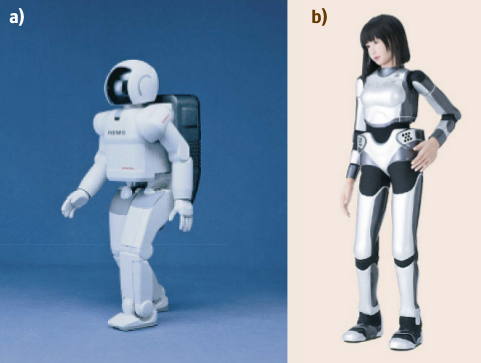
\includegraphics[scale=0.5]{images/asimov_and_HRP-4C.png}
	\caption{Diseño de robots humanoides (a) Asimov (2000); (b)HRP-4C (2009)}		
\end{figure}


		\textbf{Diseño conceptual}
El Humano cibernético o humanoide se define por las siguientes características:
\begin{itemize}
\item Tiene la apariencia y forma de un ser humano.
\item Puede caminar y moverse como un ser humano.
\item Puede interactuar con humanos usando reconocimiento de voz y de imágenes.
\end{itemize}
Tales robots pueden ser usados en la industria del entretenimiento, por ejemplo, en exhibiciones y presentaciones de moda. También se pueden usar como un simulador de humanos para evaluar dispositivos para humanos.\\

\subsection{Modelado y Control de Robots con Piernas}
	\textbf{Una Breve Historia de los Robots con piernas}\\
		Los robots con piernas controlados digitalmente empezaron a aparecer a finales de los 1960's. Entre los pioneros, Robert McGhee inicializó una serie de robots cuadrúpedos y hexápodos en \textit{University of South California}.\\

	\textbf{Dinámica del movimiento de los sistemas con piernas}\\
		Una de las mayores dificultades para hacer que un robot con extremidades camine o corra es mantener su balance: ¿Dónde debería caminar el robot?, ¿Cómo debería moverse su cuerpo a fin de moverse de manera segura en una dada dirección, incluso si hay fuertes perturbaciones?.\\ 

	\textbf{Análisis de estabilidad}\\
Para el control del sistema dinámico no lineal hay  un número de conceptos relativos para su seguridad y estabilidad los cuales son:

\begin{itemize}
\item \textit{Puntos fijos} : Representan las posturas estáticas en cuáles el robot puede estar de pie de manera segura.

\item \textit{Ciclos límites}: Proveen una natural extensión del análisis de los puntos fijos para movimientos de caminata periódica.

\item \textit{Viabilidad}: La viabilidad es un concepto de invarianza controlada, que analiza el conjunto de estados del cual el robot es capaz de mantenerse de pie. Desafortunadamente esta propiedad puede ser intratable para el cómputo.

\item \textit{Controlabilidad}: La controlabilidad provee una ligera noción de restricción de viabilidad, analizando el conjunto de estados del cual el robot es capaz de retornar a un particular punto fijo.

\item \textit{Estabilidad robusta}: Examina las propiedades del sistema considerando el "peor de los casos" de las perturbaciones. Por instancias, un controlador robusto debería ser capaz de garantizar que un punto fijo es estable incluso si la estimación de masa del tronco tiene un error del $\pm$10\%.

\item \textit{Estabilidad estocástica}: El análisis estocástico provee herramientas para investigar la probabilidad de caer. Para muchos modelos de perturbaciones en robots el sistema caerá eventualmente (con probabilidad uno), pero el análisis puede revelar la distribución del tiempo de vida metaestable.

\item \textit{Estabilidad de entrada-salida}: En este análisis se trata una particular perturbación como una entrada, un criterio de rendimiento como salida e intenta calcular una ganancia relativa o sensibilidad del rendimiento del robot debido a esta entrada.

\item \textit{Márgenes de estabilidad}: El análisis de robustez puede ser difícil. En la práctica, los diseñadores del control a menudo se conforman con que el sistema se mantenga cómodamente lejos de los límites de estabilidad determinista.		

\end{itemize}
%	\section{Aplicaciones en el juego de Futbol Soccer}
%	\section{Conceptos básicos de visión computacional}
%	\section{El filtro de Kalman}
%	\section{Trabajo relacionado}		
\chapter{ Segmentación de imágenes con base en color}
\section{Modelo de cámara Estenopeica \textit{(Pinhole)}}
De acuerdo con \cite{bradski2008learning} la visión es la detección de la luz del mundo. Esa luz empieza cuando un rayo emana desde una fuente hacia un objeto. Cuando la luz choca con el objeto, mucha de la luz es absorbida y la que no es absorbida, nosotros la podemos percibir como el color de la luz, de esta manera, la luz reflejada hace su camino hacia nuestra cámara. Esto es de particular importancia para la visión computacional.

El modelo más simple de cómo sucede el anterior fenómeno es el de la cámara estenopeica o \textit{pinhole}. Una cámara estenopeica se puede imaginar como una habitación sin ventanas en donde la luz únicamente entra por una pequeña apertura en el centro de la pared y que proyecta una imagen dentro de la habitación.

En cámara estenopeica se considera que sólo un rayo de luz entra desde un punto en particular, este punto es luego \textit{proyectado} sobre una superficie. Como resultado, la imagen en este plano (también llamado plano proyectivo), está siempre en el foco y el tamaño de la imagen se relaciona a la distancia del objeto dado por un sólo parámetro de la cámara: \textit{la distancia focal}. La principal diferencia entre la imagen real y la que aparece en una cámara Pinhole, es que la imagen aparece invertida. 
	
El punto dentro del Pinhole es reinterpretado como el centro de proyección. Para este tipo de cámara, la distancia desde la abertura del Pinhole hacia la pantalla, es precisamente la distancia focal. Como puede verse en la Figura 2.1.\\
	
\begin{figure}
	\centering		
	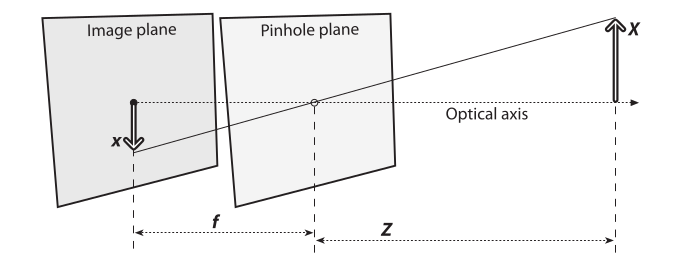
\includegraphics[scale=0.4]{images/pinhole.png}
	\caption{Esquema del modelo de cámara estenopeica  \textcolor{red}{Si copiaste la imagen de algún lado, menciona de dónde la tomaste.}}		
\end{figure}

En la Figura 2.1, $f$ es representada como la distancia focal de la cámara, $Z$ es la distancia de la cámara al objeto, $X$ es la longitud del objeto, y $x$ es la longitud de la la imagen proyectada en el plano. Dentro de la figura, se pueden ver dos triángulos semejantes los cuales cumplen que $-x/f = X/Z$, o expresado de otra manera:

\[x = -f \frac{X}{Z}\]
	
A fin de obtener ecuaciones equivalentes, pero sin signos negativos (correspondientes a la inversión de la imagen) se propone hacer un rearreglo en el cual se coloca al frente de un centro de proyección al plano proyectivo. Tal y como se ve en la Figura 2.2.
	
\begin{figure}
	\centering
	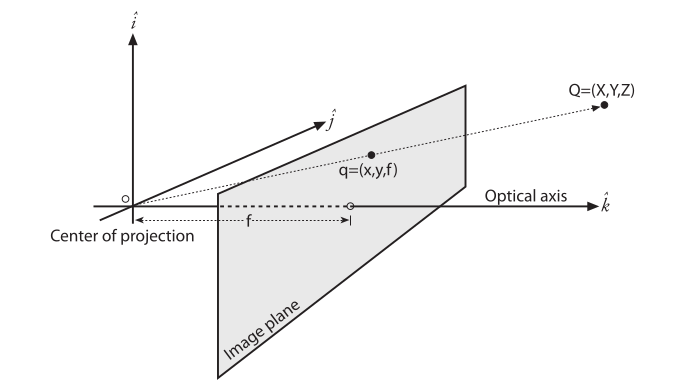
\includegraphics[scale=0.4]{images/rearreglo_pinhole.png}
    \caption{Rearreglo de una cámara estenopeica}
\end{figure} 

Con este nuevo cambio, el punto en el Pinhole es reinterpretado como el \textit{centro de proyección}, así cada rayo de luz deja un punto en el objeto distante y se dirije hacia el centro de proyección. El punto de intersección del plano proyectivo y el eje óptico es conocido como \textit{el punto principal}. El nuevo plano de imagen frontal es equivalente al anterior plano proyectivo, el el cual la imagen del objeto distante tiene exactamente el mismo tamaño que en el esquema mostrado en la Figura 2.1, la diferencia es que en este caso la imagen no queda invertida, por lo tanto la relación de los triángulos quedaría de la siguiente manera: 
\[x/f = X/Z\]

Se podría pensar que que \textit{el punto principal} es equivalente al centro de la imagen, sin embargo, este centro usualmente no está en el eje óptico, es por eso que se introducen dos nuevos parámetros, $c_{x}$ y $c_{y}$ para modelar un posible desplazamiento (perpendicular al eje óptico) del centro de coordenadas en el plano de proyección. El resultado es que un punto Q en el mundo físico cuyas coordenadas son  (X,Y,Z) es proyectado dentro de la pantalla en una localización de pixeles dada por $(x_{screen},y_{screen})$ de acuerdo con las siguientes ecuaciones:

\[x_{screen}=f_{x}(\frac{X}{Z}) \quad + c_{x},\quad y_{screen}=f_{y}(\frac{Y}{Z}) + c_{y}\]	\\


Nótese que se han introducido dos diferentes distancias focales, la razón es porque generalmente los pixeles son rectangulares.
		
\section{Corrección de la distorsión}
Desafortunadamente una verdadera cámara pinhole no es una muy buena forma de obtener imágenes porque no reune suficiente luz para crear una imagen aproximada a la real. Es por eso que los ojos y las cámaras usan lentes para reunir más luz que la que estaría disponible en un solo punto.

\subsection{Geometría básica proyectiva}
La relación que mapea los puntos $Q_{i}$ en el mundo físico con coordenadas $(X_{i},Y_{i},Z_{i})$ a los puntos en el plano de proyección con coordenadas $(x_{i},y_{i})$ es llamada una \textit{transformación proyectiva}. Cuando se trabaja con estas transformaciones es conveniente usar las \textit{coordenada homogéneas}. El plano de imagen es el espacio proyectado y tiene dos dimensiones, con lo que se pueden representar puntos en el plano como un vector tridimensional $q=(q_{1},q_{2},q_{3})$ ó $q=(x, y, w)$, en donde w es la orientación. Una forma de hacer un arreglo con los parámetros que definen a la cámara $f_{x},f_{y},c_{x}$ y $c_{y}$ dentro de una matriz de 3x3 es la llamada \textit{matriz de parámetros intrínsecos}. La proyección $q$ de los puntos del mundo físico en el plano de la imagen se puede calcular como: 
\[q=MQ\]
donde
\[q=
\begin{bmatrix}
x\\ 
y\\
w 
\end{bmatrix}\;,\;M=
\begin{bmatrix}
f_{x} & 0 & c_{x}\\ 
0     &f_{y}&c_{y} \\
0     & 0 & 1
\end{bmatrix}\;,\;Q=
\begin{bmatrix}
X\\
Y\\
Z
\end{bmatrix}
\]
\subsection{Distorsión de las lentes}
La estimación de los parámetros internos es importante en la calibración de las cámaras \cite{weng1992camera}.


Dada la manufactura y diversos factores, las lentes no son perfectas, es por eso que se introducen dos nuevos conceptos a la distorsión de las lentes, las $"Distorsiones\;radiales"$ y las $"Distorsiones\;tangenciales"$. Las primeras surgen como resultado de la forma de las lentes y las segundas como resultado del proceso de ensamblado de la camara.

%	\section{Los espacios de color RGB Y HSV}
%	\section{Operadores morfológicos}	
%	\chapter{Estimación de posición y velocidad}
%	\chapter{Implementación}
%	\chapter{Resultados}
%\bibliographystyle{apacite}
\bibliographystyle{ieeetr}
\bibliography{References}
\end{document}
